\documentclass[a4paper,12pt]{article}
\usepackage[english]{babel}
\usepackage[utf8]{inputenc}
\usepackage{amsmath}
\usepackage{amsthm}
\usepackage{amsfonts}
\usepackage{amssymb}
\usepackage{graphicx}
\usepackage{hyperref}
\usepackage{enumitem}
\usepackage{float}
\usepackage{booktabs}
\usepackage{CJKutf8}
\usepackage[colorinlistoftodos]{todonotes}
\usepackage[left=1.50cm, right=1.50cm, top=1.20cm]{geometry}
\linespread{1.5}
\usepackage{algorithm}
\usepackage{algpseudocode}
\usepackage{tikz}
\usetikzlibrary{matrix, positioning, fit}

\title{LC931---940}
\author{SS}
\date{November 2018}

\begin{document}

\maketitle

\section{931}
Given a square array of integers $A$, we want the minimum sum of a falling path through A.
\par
A falling path starts at any element in the first row, and chooses one element from each row.  The next row's choice must be in a column that is different from the previous row's column by at most one.
\paragraph{Example 1:}
\begin{flushleft}
\textbf{Input}:
\\
$M = \begin{array}{ccc}
1 & 2 & 3 \\
4 & 5 & 6 \\
7 & 8 & 9 
\end{array}$
\textbf{Output}: 12
\\
\textbf{Explanation}:
\\
The possible falling paths are:
\begin{itemize}
\item $[1,4,7], [1,4,8], [1,5,7], [1,5,8], [1,5,9]$
\item $[2,4,7], [2,4,8], [2,5,7], [2,5,8], [2,5,9], [2,6,8], [2,6,9]$
\item $[3,5,7], [3,5,8], [3,5,9], [3,6,8], [3,6,9]$
\end{itemize}
The falling path with the smallest sum is $[1,4,7]$, so the answer is 12.
\end{flushleft}
\paragraph{}
Note:Given a square array of integers $A$, we want the minimum sum of a falling path through A.
\par
A falling path starts at any element in the first row, and chooses one element from each row.  The next row's choice must be in a column that is different from the previous row's column by at most one.
\paragraph{Example 1:}
\begin{flushleft}
\textbf{Input}:
\\
$M = \begin{array}{ccc}
1 & 2 & 3 \\
4 & 5 & 6 \\
7 & 8 & 9 
\end{array}$
\\
\textbf{Output}: 12
\\
\textbf{Explanation}:
\\
The possible falling paths are:
\begin{itemize}
\item $[1,4,7], [1,4,8], [1,5,7], [1,5,8], [1,5,9]$
\item $[2,4,7], [2,4,8], [2,5,7], [2,5,8], [2,5,9], [2,6,8], [2,6,9]$
\item $[3,5,7], [3,5,8], [3,5,9], [3,6,8], [3,6,9]$
\end{itemize}
The falling path with the smallest sum is $[1,4,7]$, so the answer is 12.
\end{flushleft}
\paragraph{Note:}
\begin{flushleft}
$1 \leq |A| == |A[0]| \leq 100$
\\
$-100 <= A[i][j] <= 100$
\end{flushleft}
\subsection{Dynamic Programming Approach}
This is a very easy problem. Suppose $F$ is the \texttt{DP} array. In each position $[r,c]$ of $M$, only 3 positions in row $r-1$ can fall down to this position, i.e. $[r-1, c-1], [r-1,c], [r-1,c+1]$. Therefore, we will have
\[
F[r][c] = \min(F[r][c-1], F[r][c], F[r][c+1])
\]
Since $F[r][c]$ only depends on these three values in row $r-1$, we could use original array $A$ as the \texttt{DP} array.

\section{932 --- Beautiful Array}
For some fixed $N$, an array $A$ is beautiful if it is a permutation of the integers $1, 2, \ldots, N$, such that:
\par
For every $i < j$, there is no $k$ with $i < k < j$ such that $A[k] \times 2 = A[i] + A[j]$.
\par
Given $N$, return any beautiful array $A$.  (It is guaranteed that one exists.)
\paragraph{Example 1:}
\begin{flushleft}
\textbf{Input}: 4
\\
\textbf{Output}: $[2,1,4,3]$
\end{flushleft}
\paragraph{Example 2:}
\begin{flushleft}
\textbf{Input}: 5
\\
\textbf{Output}: $[3,1,2,5,4]$
\end{flushleft}
\subsection{Divide And Conquer}
\begin{CJK*}{UTF8}{gbsn}
假设我们已经得到了两个array $A_1$ 和 $A_2$ 都是\texttt{beautiful array}, 那么,如果其中一个都是偶数,一个都是奇数,那么合并后一定还是一个\texttt{beautiful array},因为本身两个小数组自身都已经是\texttt{beautiful array}了, 所以在$A_1, A_2$本身,是没有$i,j,k$满足 $A_1[k] \times 2 = A_1[i] + A_1[j]$ 和 $A_2[k] \times 2 = A_2[i] + A_2[j]$。
\par
如果我们在$A_1$和$A_2$里面各取一个数$A_1[i], A_2[j]$, 那么$A_1[i] + A_2[j]$就是奇数, 而$A[k]\times 2$ 是偶数, 所以这一定不存在。
\par
因此, 只要先构造一个奇数的\texttt{beautiful array}, 再构造一个偶数的\texttt{beautiful array}, 那么两者连接在一起就是一个新的\texttt{beautiful array}。
\par
接着假设已经存在一个长度为$N$的\texttt{beautiful array} $A$, 如果$A[i]\gets A[i]\times 2\; \forall i\in [0,N-1]$。在$A$中,对于任意$i<j<k$,$A[k]\times 2 \neq A[i] + A[j]$,于是就有$(A[k]\times2)\times2 \neq A[i]\times 2+ A[j]\times 2$,因此我们就得到了一个偶数的\texttt{beautiful array}。
\par
类似的,对于同样的这个$A$,$A[i] \gets 2\times A[i]-1\; \forall i \in [0, N-1]$,我们就得到了一个奇数的\texttt{beautiful array}。
\end{CJK*}
\subsubsection{Code}
In real implementation, to avoid create many temporary arrays, we can use two arrays to alternate getting the new values. Also, in C++ implementation, we can use \texttt{reserve} function to reserve $N+1$ size for these two arrays.
\setcounter{algorithm}{0}
\begin{algorithm}[H]
\caption{Divide And Conquer Approach}
\begin{algorithmic}[1]
\Procedure{$BeautifulArray$}{N}
\State $V[2]$ as $V[0]=V[1]:=\emptyset$ \Comment Two arrays, initially empty but reserve $N+1$ size
\State $V[0]\gets 1$ \Comment $N=1$, only 1 is in the array
\State $x:=0$ \Comment Get values from $V[x]$
\State $y:=1-x$ \Comment Write values to $V[y]$
\State $L:=\vert V[x]\vert$ \Comment The length of $V[x]$
\While{$L < N$}
\For{$i:=0$ \textbf{to} $L-1$}
\State $\mu_1:=2\times V[x][i] - 1$ \Comment Get the generated odd number
\If{$\mu_1 \leq N$} \Comment Only accept number not greater than $N$. (Important!)
\State $V[y] \gets V[y] + \mu_1$ \Comment Push generated odd numbers to the end of $V[y]$
\EndIf
\EndFor
\For{$i:=0$ \textbf{to} $L-1$}
\State $\mu_2:=2\times V[x][i]$ \Comment Get the generated even number
\If{$\mu_2 \leq N$} \Comment Only accept number not greater than $N$. (Important!)
\State $V[y] \gets V[y] + \mu_2$ \Comment Push generated even numbers to the end of $V[y]$
\EndIf
\State $V[x] \gets \emptyset$ \Comment Clear $V[x]$
\State $x\gets y$ 
\State $y\gets 1-x$ \Comment  Exchange $x$ with $y$
\EndFor
\EndWhile
\State \Return $V[x]$ \Comment $x\gets y$ at end of each loop. Therefore, $V[x]$ is the answer
\EndProcedure
\end{algorithmic}
\end{algorithm}
\begin{CJK*}{UTF8}{gbsn}
循环的过程相当于生成了一个树,从上到下每一层的节点数分别为$1,2,4,8,\ldots,N$。 树的高度是$\lg N$,
\end{CJK*}

\section{935 --- Knight Dialer}
We place our chess knight on any numbered key of a phone pad (indicated above), and the knight makes $N-1$ hops.  Each hop must be from one key to another numbered key.
\par
Each time it lands on a key (including the initial placement of the knight), it presses the number of that key, pressing $N$ digits total.
\par
How many distinct numbers can you dial in this manner?
\par
Since the answer may be large, output the answer modulo $10^9 + 7$.
\paragraph{Example 1:}
\begin{flushleft}
\textbf{Input}: 1
\\
\textbf{Output}: 10
\end{flushleft}
\paragraph{Example 2:}
\begin{flushleft}
 \textbf{Input}: 2
 \\
 \textbf{Output}: 20
 \end{flushleft} 
\paragraph{Example 3:}
\begin{flushleft}
\textbf{Input}: 3
\\
\textbf{Output}: 46
\end{flushleft}
\subsection{Dynamic Programming}
\begin{figure}[H]
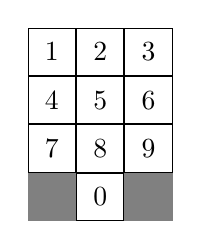
\begin{tikzpicture}
[keynode/.style={draw, rectangle, minimum size=6mm}]
\node (){};
\node [keynode] (1) {1}; 
\node [keynode, right=0mm of 1.east] (2) {2}; 
\node [keynode, right=0mm of 2.east] (2) {3}; 
\node [keynode, below=0mm of 1.south] (4) {4};
\node [keynode, right=0mm of 4.east] (5) {5}; 
\node [keynode, right=0mm of 5.east] (6) {6}; 
\node [keynode, below=0mm of 4.south] (7) {7};
\node [keynode, right=0mm of 7.east] (8) {8}; 
\node [keynode, right=0mm of 8.east] (9) {9};
\node [keynode, fill, color=gray, below=0mm of 7.south] (a) {};
\node [keynode, right=0mm of a.east] (0) {0}; 
\node [keynode, fill, color=gray, right=0mm of 0.east] (b) {};
\end{tikzpicture}
\end{figure}
We can observe that each key can only jump to fixed keys. This fulfills a recursive structure. Let $F(\alpha, n)$ be the number of ways to dial an $n$ digit number by the knight. The knight starts at key $\alpha$. For example, the knight can only jump to 6 and 8 from key 1. Therefore, $F(1, n) = F(6, n-1) + F(8, n-1)$.
\par
For each iteration, we count the appearances of keys would appear in the next move, i.e, we update $F(\alpha, n)$ while n iterates from 1 to $N-1$. To facilitate counting in each iteration, we use two arrays $\Omega_1$ and $\Omega_2$. Among them, $\Omega_1$ is the counts of each number in the last iteration while $\Omega_2$ is for the current iteration. After each iteration, we swap $\Omega_1$ and $\Omega_2$. Also, at the beginning of each iteration, reset $\Omega_2$ to zero for each key.
\subsubsection{Code}
\setcounter{algorithm}{0}
\begin{algorithm}[H]
\caption{Dynamic Programming Approach}
\begin{algorithmic}[1]
\Procedure{KnightDialer}{$N$}
\State $\Omega_1$ as $\Omega_1[0]=\ldots=\Omega_1[9]:=1$ \Comment Count of each key in the last iteration
\State $\Omega_2$ as $\Omega_2[0]=\ldots=\Omega_2[9]:=0$ \Comment Count of each key in current iteration
\For{$i:=1$ \textbf{to} $N-1$}
\State $\Omega_2[i] \gets 0, \; i\in [0,9]$ \Comment Reset current count of each key
\For{$k:=0$ \textbf{to} $9$}
\For{$n \in M[k]$} \Comment Iterate each next key from $k$ \label{935M}
\State $\Omega_2[n] \gets \Omega_2[n] + \Omega_1[k]$
\EndFor
\EndFor
\State $\Omega_1 \leftrightarrow \Omega_2$ \Comment Swap $\Omega_1$ and $\Omega_2$
\EndFor
\State $\delta:=0$ \Comment The result count
\For{$i:=0$ \textbf{to} $9$}
\State $\delta\gets\delta+\Omega_1[i]$
\EndFor
\State \Return $\delta$
\EndProcedure
\end{algorithmic}
\end{algorithm}
In line [\ref{935M}], $M$ is a hash map with relationship between each key and next keys by the knight to take one jump. By observing the keypad, we will have
\[
\begin{array}{lll}
1 \longrightarrow (6, 8) & 2 \longrightarrow (7, 9)\ & 3 \longrightarrow (4, 8) \\
4 \longrightarrow (0,3,9) & 5 \longrightarrow \varnothing & 6 \longrightarrow (0,1,7) \\
7 \longrightarrow (2,6) & 8 \longrightarrow (1,3) & 9 \longrightarrow (2,4) \\
0 \longrightarrow (4,6) & & \\
\end{array}
\]

\section{934 --- Shortest Bridge}
In a given 2D binary array $A$, there are two islands.  (An island is a 4-directionally connected group of 1s not connected to any other 1s.)
\par
Now, we may change 0s to 1s so as to connect the two islands together to form 1 island.
\par
Return the smallest number of 0s that must be flipped.  (It is guaranteed that the answer is at least 1.)
\paragraph{Example 1:}
\begin{flushleft}
\textbf{Input}: 
\begin{figure}[H]
\begin{tikzpicture}
\matrix[matrix of nodes]
{
 0 &  1 \\
 1 & 0 \\
};
\end{tikzpicture}
\end{figure}
\textbf{Output}: 1
\end{flushleft}
\paragraph{Example 2:}
\begin{flushleft}
\textbf{Input}:
\begin{figure}[H]
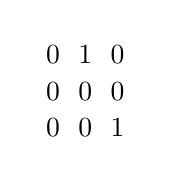
\begin{tikzpicture}
\matrix[matrix of nodes]
{
0 & 1 & 0 \\ 
0 & 0 & 0 \\
0 & 0 & 1\\
};
\end{tikzpicture}
\end{figure}
\end{flushleft}
\textbf{Output}: 2
\paragraph{Example 3:}
\begin{flushleft}
\textbf{Input}:
\begin{figure}[H]
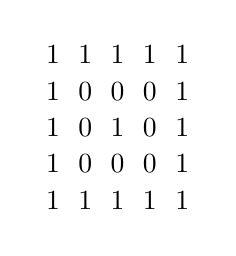
\begin{tikzpicture}
\matrix[matrix of nodes]
{
1 & 1 & 1 & 1 & 1\\
1 & 0 & 0 & 0 & 1\\
1 & 0 & 1 & 0 & 1\\
1 & 0 & 0 & 0 & 1\\
1 & 1 & 1 & 1 & 1 \\
};
\end{tikzpicture}
\end{figure}
\textbf{Output}: 1
\end{flushleft}
\paragraph{Note:}
\begin{flushleft}
$1\leq |A| = |A[0]| \leq 100$
\\
$A[i][j] = 0/1$
\end{flushleft}
\subsection{Depth First Paint And Breadth First Grow}
Conceptually, this method is very straightforward: find both islands, paint with two numbers. Then for one of the islands, keep \textit{growing} it by 1 until we touch the second island.
\par
We can use a depth-first search to find the islands, and a breadth-first search to \textit{grow} one of them. This leads to a verbose but correct solution.
\par
To find both islands, look for a square with a 1 we haven't visited, and dfs to get the component of that region. Paint this region with the given color. Do this twice. After, we have two components source and target. Both are painted with two different numbers say 2 and 3.
\par
To find the shortest bridge, do a BFS from the nodes source, say the component painted with number 2. In the process of growing of island 2, if we find any node is in island 3, the shortest distance then is found. To facilitate the depth information during \textit{growing}, we can add current node's depth information besides the row and column position.
\subsection{Code}
In the following procedure, we use a structure contains row, column and depth information of a cell during \textit{growing} process. The input $A$ is $N\times N$ matrix.
\setcounter{algorithm}{0}
\begin{algorithm}[H]
\caption{BFS And DFS Approach}
\begin{algorithmic}[1]
\Procedure{ShortestBridge}{$A, N$}
\State $\pi:=2$ \Comment The color to paint the connected component
\For{$r:=0$ \textbf{to} $N-1$}
\For{$c:=0$ \textbf{to} $N-1$}
\If{$A[r][c] = 1$}
\State $\Gamma(A, N, r, c, \pi)$
\State $\pi \gets \pi+1$ \Comment The color to paint next connected component
\EndIf
\EndFor
\EndFor
\algstore{934algo}
\end{algorithmic}
\end{algorithm}
\begin{algorithm}[H]
\begin{algorithmic}[1]
\algrestore{934algo}
\State $Q:=\emptyset$ \Comment An empty queue
\For{$r:=0$ \textbf{to} $N-1$}
\For{$c:=0$ \textbf{to} $N-1$}
\If{$A[r][c] = 2$} \Comment The starting island is the color 2
\State $Q \gets Q + (r, c, 0)$ \Comment Push $(r,c)$ with its depth 0 to $Q$
\EndIf
\EndFor
\EndFor
\State $\delta$ as $\delta[0]:=(0,1), \delta[1]:=(0,-1), \delta[2]:=(1,0), \delta[3]:=(-1,0)$ \Comment The 4 direction offsets
\While{$Q\neq \emptyset$} \Comment Starting the growing process \label{934While}
\State $(r, c, d) := Q[0]$ \Comment Get the front of $Q$
\State $Q\gets Q\setminus Q[0]$  \Comment Pop front of $Q$
\For{$i:=0$ \textbf{to} $3$} \label{934fordirection}
\State $\Bar{r}:=r + \delta[0][0]$ \Comment The row of next move
\State $\Bar{c}:=c + \delta[0][1]$ \Comment The column of next move
\If{$0\leq \Bar{r}<N$ \textbf{and} $0\leq \Bar{c}<N$ \textbf{and} $A[\Bar{r}][\Bar{c}]\neq 2$} \Comment $(\Bar{r}, \Bar{c})$ is not in island 2 \label{934If1}
\If{$A[\Bar{r}][\Bar{c}] = 3$} \Comment $(\Bar{r}, \Bar{c})$ is in island 3
\State \Return $d$ \Comment The current depth is the result
\EndIf
\If{$A[\Bar{r}][\Bar{c}] = 0$} \Comment $(\Bar{r}, \Bar{c})$ is water
\State $A[\Bar{r}][\Bar{c}]\gets 2$ \Comment Expand island 2 to $(\Bar{r}, \Bar{c})$
\State $Q\gets Q + (\Bar{r},\Bar{c},d+1)$ \Comment Push $(\Bar{r}, \Bar{c})$ and related depth into $Q$
\EndIf 
\EndIf \Comment End[\ref{934If1}]
\EndFor \Comment End[\ref{934fordirection}] 
\EndWhile \Comment End[\ref{934While}]
\State \Return $-1$ \Comment Cannot find the path from island 2 to island 3
\EndProcedure
\end{algorithmic}
\end{algorithm}
Function $\Gamma$ color the connected component with color $\pi$ starting with position $(r,c)$
\begin{algorithm}[H]
\caption{Recursive Color Connected Component}
\begin{algorithmic}[1]
\Function{$\Gamma$}{$A, N, r, c, \pi$}
\State $A[r][c] = \pi$
\State $\delta$ as $\delta[0]:=(0,1), \delta[1]:=(0,-1), \delta[2]:=(1,0), \delta[3]:=(-1,0)$ \Comment The 4 direction offsets
\For{$i:=0$ \textbf{to} $3$}
\State $\Bar{r}:=r + \delta[0][0]$ \Comment The row of next move
\State $\Bar{c}:=c + \delta[0][1]$ \Comment The column of next move
\If{$0\leq \Bar{r}<N$ \textbf{and} $0\leq \Bar{c}<N$ \textbf{and} $A[\Bar{r}][\Bar{c}]=1$}
\State $\Gamma(A, N, \Bar{r}, \Bar{c}, \pi)$ \Comment Depth first coloring connected cells
\EndIf
\EndFor
\EndFunction
\end{algorithmic}
\end{algorithm}

\section{936 --- Stamping The Sequence}
You want to form a target string with lowercase letters $T$ with length $L$.
\par
At the beginning, $T$ is filled with \texttt{?}.  You also have a stamp of lowercase letters $S$ with length $N$.
\par
On each turn, you may place the stamp over the sequence, and replace every letter in the sequence with the corresponding letter from the stamp.  You can make up to $10 \times L$ turns.
\par
For example, if the initial sequence is \texttt{?????}, and $S$ is \texttt{abc},  then you may make \texttt{abc??}, \texttt{?abc?} or \texttt{??abc} in the first turn.  (Note that the stamp must be fully contained in the boundaries of the sequence in order to stamp.)
\par
If the sequence $T$ is possible to stamp, then return an array of the index of the left-most letter being stamped at each turn. If $T$ is impossible to stamp, return an empty array.
\par
For example, if $T$ is \texttt{ababc}, and $S$ is \texttt{abc}, then we could return the answer $[0, 2]$, corresponding to the moves $\texttt{?????} \longrightarrow \texttt{abc??} \longrightarrow \texttt{ababc}$.
\par
Also, if $T$ is possible to stamp, it is guaranteed it is possible to stamp within $10 \times L$ moves.  Any answers specifying more than this number of moves will not be accepted.
\subsection{Reverse Operation}
We can find the stamp process by reversing the operation, i.e., starting from the target and fill with $\ast$ to see if we can fill the target with $\ast$
\par
The letters which stamped later will cover the letters stamped before and we really don't care about the letters which are covered. For example, suppose $T$ is \texttt{aabcaca}. Since we do not care about the letters which are coverd by others, so we can apply a $\ast$ match any letters. Then the reverse process is shown as below:
\[
\texttt{aabcaca} \Rightarrow \texttt{a}\ast\ast\ast\ast\texttt{ca} \Rightarrow \ast\ast\ast\ast\ast\texttt{ca} \Rightarrow \ast\ast\ast\ast\ast\ast\ast
\]
\subsection{Code}
Procedure \texttt{MovesToStamp} returns a array contains the positions that put $S$ to form $T$. $S$ length is $N$ while $T$ is $L$.
\setcounter{algorithm}{0}
\begin{algorithm}[H]
\caption{Reverse Process Approach}
\begin{algorithmic}[1]
\Procedure{MovesToStamp}{$S, N, T, L$}
\State $F:=\underbrace{\ast\ldots\ast}_{L}$ \Comment $F$ is the final string filled with all $\ast$
\State $V:=\emptyset$ \Comment The position array 
\While{$T\neq F$}
\State $p:=\Pi(S, T)$ \Comment Get the position that can fill $\ast$
\If{$p=-1$}
\State \Return $\emptyset$ \Comment Cannot stamp $S$ to $T$
\Else
\State $V\gets V+p$ \Comment Add $p$ to $V$
\EndIf
\EndWhile
\State Reverse $V$ \Comment Since the process is reversed
\State \Return $V$
\EndProcedure
\end{algorithmic}
\end{algorithm}

Function $\Pi$ get the position from where $\ast$ can be filled in $T$ by comparing $S$ with $T$. If $T[i]=\ast$, it means $T[i]$ still matches $S[j]$
\begin{algorithm}[H]
\caption{Get The Fill Position}
\begin{algorithmic}[1]
\Function{$\Pi$}{$S, N, T, L$}
\For{$i:=0$ \textbf{to} $N-1$} \label{936for1}
\State $j:=i$\Comment The index in $T$
\State $k:=0$ \Comment The index in $S$
\State $\alpha:=0$ \Comment $0/1$ boolean variable indicates if $T$ match $S$ on a lowercase letter not $\ast$
\While{$k < N$ \textbf{and} $j < L$} \label{936While1}
\If{$S[k]=T[j]$ \textbf{or} $T[j] = \ast$} \Comment Either match stamp or is $\ast$
\State $k\gets k+1, j\gets j+1$
\If{$S[k] = T[i]$} \Comment $S$ and $T$ match on a lowercase letter
\State $\alpha\gets 1$
\EndIf
\EndIf
\EndWhile \Comment End[\ref{936While1}]
\If{$k=N$ \textbf{and} $\alpha=1$} \Comment $S[0\ldots k-1]$ matches $T[i\ldots j-1]$ on at least one letter
\State $T[i\ldots j-1] \gets \underbrace{\ast\ldots\ast}_{N}$ \Comment $j-i = N$ so fill $T[i\ldots j-1]$ with $\ast$
\State \Return $i$ \Comment Position $i$ can fill $\ast$
\EndIf
\EndFor \Comment End[\ref{936for1}]
\State \Return $-1$ \Comment Cannot find any position that can fill $\ast$
\EndFunction
\end{algorithmic}
\end{algorithm}
To optimize more, we can use \texttt{KMP} algorithm to find all matched substrings in $T$ and fill them with $\ast$. Then use the same process as above to fill the remaining positions with $\ast$. 
\end{document}
